% Practice Test 08 — Florida Edition
% Questions: 30 (21 MC + 9 SA)
% Generated by scripts/generate_practice_tests.py

\begin{practiceQuestion}{1-3-q13}{mc}
\begin{questionText}
The table shows a proportional relationship. Find the missing value.

\begin{center}
\begin{tabular}{|c|c|}
\hline $x$ & $y$ \\ \hline $4$ & $14$ \\ $6$ & $?$ \\ $10$ & $35$ \\ \hline
\end{tabular}
\end{center}
\end{questionText}
\choiceA{$18$}
\choiceB{$20$}
\choiceC{$21$}
\choiceD{$24$}
\correctAnswer{C}
\explanation{$k = \frac{14}{4} = 3.5$. Missing value: $y = 3.5 \times 6 = 21$. Check: $\frac{35}{10} = 3.5$ \checkmark.}
\end{practiceQuestion}

\begin{practiceQuestion}{1-6-q21}{sa}
\begin{questionText}
A scale drawing uses $1$ cm $= 4.5$ m. If a building is $27$ m tall, how tall is it in the drawing?
\end{questionText}
\correctAnswer{$6$ cm}
\explanation{$\frac{1}{4.5} = \frac{x}{27}$. Cross-multiply: $4.5x = 27$, so $x = 6$ cm.}
\end{practiceQuestion}

\begin{practiceQuestion}{2-1-q26}{gmc}
\begin{questionText}
The $10 \times 10$ grid below has some squares shaded. What percent of the grid is shaded?

\begin{center}
\begin{tikzpicture}[scale=0.35]
  \foreach \x in {0,...,9} {
    \foreach \y in {0,...,9} {
      \draw[gray!50] (\x,\y) rectangle (\x+1,\y+1);
    }
  }
  % Shade 35 squares (rows 0-2 full = 30, plus 5 in row 3)
  \foreach \x in {0,...,9} {
    \foreach \y in {0,...,2} {
      \fill[funBlue!40] (\x,\y) rectangle (\x+1,\y+1);
      \draw[gray!50] (\x,\y) rectangle (\x+1,\y+1);
    }
  }
  \foreach \x in {0,...,4} {
    \fill[funBlue!40] (\x,3) rectangle (\x+1,4);
    \draw[gray!50] (\x,3) rectangle (\x+1,4);
  }
\end{tikzpicture}
\end{center}
\end{questionText}
\choiceA{$25\%$}
\choiceB{$30\%$}
\choiceC{$35\%$}
\choiceD{$40\%$}
\correctAnswer{C}
\explanation{The grid has $100$ squares total. Count the shaded squares: $3$ full rows of $10 = 30$, plus $5$ more $= 35$. So $35\%$ is shaded.}
\end{practiceQuestion}

\begin{practiceQuestion}{2-2-q10}{mc}
\begin{questionText}
$96$ is $80\%$ of what number?
\end{questionText}
\choiceA{$76.8$}
\choiceB{$100$}
\choiceC{$116$}
\choiceD{$120$}
\correctAnswer{D}
\explanation{$\frac{96}{w} = \frac{80}{100}$. Cross-multiply: $80w = 9600$. Divide: $w = 120$.}
\end{practiceQuestion}

\begin{practiceQuestion}{2-6-q17}{mc}
\begin{questionText}
Jake deposits $\$2{,}500$ at $3\%$ simple interest. After how many years will the total reach $\$2{,}875$?
\end{questionText}
\choiceA{$3$ years}
\choiceB{$4$ years}
\choiceC{$5$ years}
\choiceD{$6$ years}
\correctAnswer{C}
\explanation{Interest needed: $2{,}875 - 2{,}500 = \$375$. $375 = 2{,}500 \times 0.03 \times t$ → $375 = 75t$ → $t = 5$ years.}
\end{practiceQuestion}

\begin{practiceQuestion}{2-7-q27}{gmc}
\begin{questionText}
The bar graph shows the estimated and actual heights of three trees. Which tree has the greatest percent error?

\begin{center}
\begin{tikzpicture}[scale=0.5]
  \draw[thick,->] (0,0) -- (0,7) node[above]{\small Height (ft)};
  \draw[thick,->] (0,0) -- (10.5,0);
  % Tree A: est 20, actual 25
  \fill[funBlue!60] (0.5,0) rectangle (1.5,4);
  \fill[funGreen!60] (1.5,0) rectangle (2.5,5);
  % Tree B: est 15, actual 12
  \fill[funBlue!60] (3.5,0) rectangle (4.5,3);
  \fill[funGreen!60] (4.5,0) rectangle (5.5,2.4);
  % Tree C: est 30, actual 28
  \fill[funBlue!60] (6.5,0) rectangle (7.5,6);
  \fill[funGreen!60] (7.5,0) rectangle (8.5,5.6);
  % Labels
  \node[below,font=\small] at (1.5,0) {Tree A};
  \node[below,font=\small] at (4.5,0) {Tree B};
  \node[below,font=\small] at (7.5,0) {Tree C};
  \foreach \y/\lab in {1/5,2/10,3/15,4/20,5/25,6/30} {
    \draw (-0.1,\y) -- (0.1,\y) node[left,font=\small,xshift=-2pt] {\lab};
  }
  % Values
  \node[above,font=\scriptsize,funBlue] at (1,4) {$20$};
  \node[above,font=\scriptsize,funGreen!80!black] at (2,5) {$25$};
  \node[above,font=\scriptsize,funBlue] at (4,3) {$15$};
  \node[above,font=\scriptsize,funGreen!80!black] at (5,2.4) {$12$};
  \node[above,font=\scriptsize,funBlue] at (7,6) {$30$};
  \node[above,font=\scriptsize,funGreen!80!black] at (8,5.6) {$28$};
  % Legend
  \fill[funBlue!60] (0.5,6.8) rectangle (1,7.2);
  \node[right,font=\scriptsize] at (1.1,7) {Estimated};
  \fill[funGreen!60] (3.5,6.8) rectangle (4,7.2);
  \node[right,font=\scriptsize] at (4.1,7) {Actual};
\end{tikzpicture}
\end{center}
\end{questionText}
\choiceA{Tree A ($20\%$)}
\choiceB{Tree B ($25\%$)}
\choiceC{Tree C ($7.1\%$)}
\choiceD{Trees A and B are tied}
\correctAnswer{B}
\explanation{A: $|20-25|/25 = 20\%$. B: $|15-12|/12 = 25\%$. C: $|30-28|/28 \approx 7.1\%$. Tree B has the greatest error.}
\end{practiceQuestion}

\begin{practiceQuestion}{3-2-q04}{mc}
\begin{questionText}
What is $9 + (-14)$?
\end{questionText}
\choiceA{$23$}
\choiceB{$-23$}
\choiceC{$-5$}
\choiceD{$5$}
\correctAnswer{C}
\explanation{Different signs: $14 - 9 = 5$. The larger absolute value ($14$) is negative, so the answer is $-5$.}
\end{practiceQuestion}

\begin{practiceQuestion}{3-3-q12}{mc}
\begin{questionText}
What is $(-3) - 5 - (-10)$?
\end{questionText}
\choiceA{$-18$}
\choiceB{$2$}
\choiceC{$-2$}
\choiceD{$12$}
\correctAnswer{B}
\explanation{Rewrite: $(-3) + (-5) + 10$. Add negatives: $-3 + (-5) = -8$. Then $-8 + 10 = 2$.}
\end{practiceQuestion}

\begin{practiceQuestion}{4-4-q25}{sa}
\begin{questionText}
Show that $4(5x + 3)$ and $20x + 12$ are equivalent by expanding.
\end{questionText}
\correctAnswer{$4(5x + 3) = 4 \times 5x + 4 \times 3 = 20x + 12$}
\explanation{Distribute $4$: $4 \times 5x = 20x$ and $4 \times 3 = 12$. So $4(5x + 3) = 20x + 12$ \checkmark. They are equivalent.}
\end{practiceQuestion}

\begin{practiceQuestion}{4-5-q03}{mc}
\begin{questionText}
When subtracting $(4x - 1)$ from $(7x + 3)$, the first step is to:
\end{questionText}
\choiceA{Add $4x$ and $7x$}
\choiceB{Distribute the negative sign to both $4x$ and $-1$}
\choiceC{Subtract $3$ from $1$}
\choiceD{Multiply $7x$ by $-1$}
\correctAnswer{B}
\explanation{$(7x + 3) - (4x - 1)$ requires distributing the negative to every term in the second expression: $7x + 3 - 4x + 1$.}
\end{practiceQuestion}

\begin{practiceQuestion}{5-3-q30}{gsa}
\begin{questionText}
Four friends go to a museum. Each person pays for a ticket and a $\$3$ audio guide. The total for all four people is $\$68$. The equation $4(t + 3) = 68$ represents this situation, where $t$ is the ticket price. Use the model below to find $t$.

\begin{center}
\begin{tikzpicture}[scale=0.6]
  % 4 bars
  \foreach \i in {0,...,3} {
    \draw[thick,fill=funBlue!20] (0,\i*1.2) rectangle (6,\i*1.2+0.9);
    \draw[thick,fill=funOrange!30] (6,\i*1.2) rectangle (8,\i*1.2+0.9);
    \node at (3,\i*1.2+0.45) {$t$};
    \node at (7,\i*1.2+0.45) {$\$3$};
  }
  \node[left] at (-0.3,1.8) {$4$ people};
  \draw[decorate,decoration={brace,amplitude=6pt}] (8.3,4.5) -- (8.3,0);
  \node[right] at (8.7,2.25) {$\$68$};
\end{tikzpicture}
\end{center}
\end{questionText}
\correctAnswer{$t = \$14$}
\explanation{$4(t + 3) = 68$. Divide by $4$: $t + 3 = 17$. Subtract $3$: $t = 14$. Each ticket costs $\$14$.}
\end{practiceQuestion}

\begin{practiceQuestion}{5-4-q19}{sa}
\begin{questionText}
Solve $\dfrac{3x}{4} - 2 = 7$.
\end{questionText}
\correctAnswer{$x = 12$}
\explanation{Add $2$: $\frac{3x}{4} = 9$. Multiply by $4$: $3x = 36$. Divide by $3$: $x = 12$. Check: $\frac{3(12)}{4} - 2 = 9 - 2 = 7$ \checkmark.}
\end{practiceQuestion}

\begin{practiceQuestion}{5-5-q21}{sa}
\begin{questionText}
Write an inequality: ``A number $x$ divided by $4$, minus $3$, is at least $2$.'' Then solve.
\end{questionText}
\correctAnswer{$\dfrac{x}{4} - 3 \geq 2$; $x \geq 20$}
\explanation{$\frac{x}{4} - 3 \geq 2$. Add $3$: $\frac{x}{4} \geq 5$. Multiply by $4$: $x \geq 20$.}
\end{practiceQuestion}

\begin{practiceQuestion}{5-6-q07}{mc}
\begin{questionText}
The graph of an inequality has an open circle at $-1$ and is shaded to the left. Which inequality matches?
\end{questionText}
\choiceA{$x \leq -1$}
\choiceB{$x < -1$}
\choiceC{$x \geq -1$}
\choiceD{$x > -1$}
\correctAnswer{B}
\explanation{Open circle means $-1$ is not included, shading left means less than: $x < -1$.}
\end{practiceQuestion}

\begin{practiceQuestion}{6-2-q02}{mc}
\begin{questionText}
A blueprint uses $1$ cm $= 4$ m. You want to redraw it at $1$ cm $= 8$ m. A wall that is $10$ cm on the original becomes how long on the new drawing?
\end{questionText}
\choiceA{$5$ cm}
\choiceB{$10$ cm}
\choiceC{$20$ cm}
\choiceD{$40$ cm}
\correctAnswer{A}
\explanation{Scale ratio: $\frac{4}{8} = \frac{1}{2}$. New length: $10 \times \frac{1}{2} = 5$ cm. A larger scale (more real units per cm) shrinks the drawing.}
\end{practiceQuestion}

\begin{practiceQuestion}{6-4-q24}{sa}
\begin{questionText}
You are given two sides ($5$ cm and $7$ cm) and the included angle ($90°$). Is the resulting triangle unique? What type of triangle is it?
\end{questionText}
\correctAnswer{Yes, unique; it is a right triangle}
\explanation{SAS produces a unique triangle. The included angle of $90°$ makes it a right triangle with legs $5$ cm and $7$ cm.}
\end{practiceQuestion}

\begin{practiceQuestion}{6-5-q28}{gmc}
\begin{questionText}
The diagram shows a triangular prism. A cut is made parallel to the triangular base (shown as the shaded region). What is the cross-section?

\begin{center}
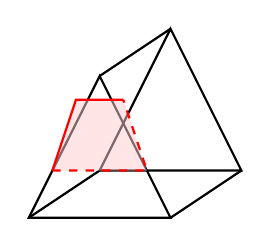
\begin{tikzpicture}[scale=0.6]
  % Front triangle
  \draw[thick] (0,0) -- (3,0) -- (1.5,3) -- cycle;
  % Back triangle
  \draw[thick] (1.5,1) -- (4.5,1) -- (3,4) -- cycle;
  % Connecting edges
  \draw[thick] (0,0) -- (1.5,1);
  \draw[thick] (3,0) -- (4.5,1);
  \draw[thick] (1.5,3) -- (3,4);
  % Cross section
  \fill[red!20,opacity=0.5] (0.5,1) -- (2.5,1) -- (2,2.5) -- (1,2.5) -- cycle;
  \draw[thick,red,dashed] (0.5,1) -- (2.5,1) -- (2,2.5);
  \draw[thick,red] (0.5,1) -- (1,2.5) -- (2,2.5);
\end{tikzpicture}
\end{center}
\end{questionText}
\choiceA{Rectangle}
\choiceB{Triangle}
\choiceC{Circle}
\choiceD{Hexagon}
\correctAnswer{B}
\explanation{A cut parallel to the base of a prism gives a shape congruent to the base. Since the base is a triangle, the cross-section is a triangle.}
\end{practiceQuestion}

\begin{practiceQuestion}{6-6-q15}{mc}
\begin{questionText}
Which pair of angles is complementary?
\end{questionText}
\choiceA{$50°$ and $130°$}
\choiceB{$55°$ and $35°$}
\choiceC{$60°$ and $60°$}
\choiceD{$45°$ and $135°$}
\correctAnswer{B}
\explanation{Complementary angles sum to $90°$. Only $55 + 35 = 90$.}
\end{practiceQuestion}

\begin{practiceQuestion}{7-1-q04}{mc}
\begin{questionText}
Which of the following best describes the circumference of a circle?
\end{questionText}
\choiceA{The distance from the center to the edge}
\choiceB{The distance across the circle through the center}
\choiceC{The distance around the circle}
\choiceD{The area inside the circle}
\correctAnswer{C}
\explanation{The circumference is the distance around (perimeter of) a circle.}
\end{practiceQuestion}

\begin{practiceQuestion}{7-5-q17}{mc}
\begin{questionText}
A paint company needs to paint the outside of a box that is $3$ m by $2$ m by $1$ m. Each can of paint covers $5$ m$^2$. How many cans are needed?
\end{questionText}
\choiceA{$3$}
\choiceB{$4$}
\choiceC{$5$}
\choiceD{$6$}
\correctAnswer{C}
\explanation{$SA = 2(3 \times 2) + 2(3 \times 1) + 2(2 \times 1) = 12 + 6 + 4 = 22$ m$^2$. Cans: $22 \div 5 = 4.4$. Round up to $5$ cans.}
\end{practiceQuestion}

\begin{practiceQuestion}{7-6-q26}{gmc}
\begin{questionText}
What is the volume of the rectangular prism shown?

\begin{center}
\begin{tikzpicture}[scale=0.4]
  % Front face
  \draw[thick,funBlue,fill=funBlue!10] (0,0) -- (7,0) -- (7,4) -- (0,4) -- cycle;
  % Top face
  \draw[thick,funBlue,fill=funBlue!20] (0,4) -- (2.5,6) -- (9.5,6) -- (7,4) -- cycle;
  % Right face
  \draw[thick,funBlue,fill=funBlue!15] (7,0) -- (9.5,2) -- (9.5,6) -- (7,4) -- cycle;
  % Labels
  \draw[thick,funRed,<->] (0,-0.7) -- (7,-0.7);
  \node[below,funRed] at (3.5,-0.7) {$7$ cm};
  \draw[thick,funRed,<->] (10,2) -- (10,6);
  \node[right,funRed] at (10,4) {$4$ cm};
  \draw[thick,funRed,<->] (7,-0.7) -- (9.5,1.3);
  \node[below right,funRed] at (8.25,0.1) {$3$ cm};
\end{tikzpicture}
\end{center}
\end{questionText}
\choiceA{$14$ cm$^3$}
\choiceB{$42$ cm$^3$}
\choiceC{$84$ cm$^3$}
\choiceD{$168$ cm$^3$}
\correctAnswer{C}
\explanation{$V = 7 \times 3 \times 4 = 84$ cm$^3$.}
\end{practiceQuestion}

\begin{practiceQuestion}{7-7-q20}{sa}
\begin{questionText}
A cylindrical jar has a diameter of $12$ cm and a height of $15$ cm. What is its volume? Use $\pi \approx 3.14$.
\end{questionText}
\correctAnswer{$1{,}695.6$ cm$^3$}
\explanation{$r = 6$ cm. $V = 3.14 \times 36 \times 15 = 1{,}695.6$ cm$^3$.}
\end{practiceQuestion}

\begin{practiceQuestion}{8-1-q16}{mc}
\begin{questionText}
Why is a convenience sample (e.g., surveying your friends) usually not a good way to learn about a population?
\end{questionText}
\choiceA{It is too expensive}
\choiceB{It takes too long}
\choiceC{It is likely biased and not representative}
\choiceD{It includes too many people}
\correctAnswer{C}
\explanation{Convenience samples are easy but likely biased because they don't give everyone an equal chance.}
\end{practiceQuestion}

\begin{practiceQuestion}{8-3-q30}{gsa}
\begin{questionText}
The dot plots show quiz scores for two classes (out of $10$).

\begin{center}
\begin{tikzpicture}[scale=0.6]
  % Class X
  \node[left,font=\small\bfseries] at (3.5,2) {Class X};
  \draw[thick,->] (3.5,0) -- (11.5,0);
  \foreach \x in {4,5,...,10} {
    \draw (\x,0.1) -- (\x,-0.1);
    \node[below,font=\small] at (\x,0) {$\x$};
  }
  % Class X data: 5(1),6(2),7(4),8(5),9(3),10(1) = 16 students
  \fill[funBlue] (5,0.35) circle (0.13);
  \fill[funBlue] (6,0.35) circle (0.13); \fill[funBlue] (6,0.65) circle (0.13);
  \fill[funBlue] (7,0.35) circle (0.13); \fill[funBlue] (7,0.65) circle (0.13); \fill[funBlue] (7,0.95) circle (0.13); \fill[funBlue] (7,1.25) circle (0.13);
  \fill[funBlue] (8,0.35) circle (0.13); \fill[funBlue] (8,0.65) circle (0.13); \fill[funBlue] (8,0.95) circle (0.13); \fill[funBlue] (8,1.25) circle (0.13); \fill[funBlue] (8,1.55) circle (0.13);
  \fill[funBlue] (9,0.35) circle (0.13); \fill[funBlue] (9,0.65) circle (0.13); \fill[funBlue] (9,0.95) circle (0.13);
  \fill[funBlue] (10,0.35) circle (0.13);

  % Class Y
  \node[left,font=\small\bfseries] at (3.5,5.5) {Class Y};
  \draw[thick,->] (3.5,3.5) -- (11.5,3.5);
  \foreach \x in {4,5,...,10} {
    \draw (\x,3.6) -- (\x,3.4);
  }
  % Class Y data: 4(2),5(3),6(4),7(3),8(2),9(1),10(1) = 16 students
  \fill[funGreen] (4,3.85) circle (0.13); \fill[funGreen] (4,4.15) circle (0.13);
  \fill[funGreen] (5,3.85) circle (0.13); \fill[funGreen] (5,4.15) circle (0.13); \fill[funGreen] (5,4.45) circle (0.13);
  \fill[funGreen] (6,3.85) circle (0.13); \fill[funGreen] (6,4.15) circle (0.13); \fill[funGreen] (6,4.45) circle (0.13); \fill[funGreen] (6,4.75) circle (0.13);
  \fill[funGreen] (7,3.85) circle (0.13); \fill[funGreen] (7,4.15) circle (0.13); \fill[funGreen] (7,4.45) circle (0.13);
  \fill[funGreen] (8,3.85) circle (0.13); \fill[funGreen] (8,4.15) circle (0.13);
  \fill[funGreen] (9,3.85) circle (0.13);
  \fill[funGreen] (10,3.85) circle (0.13);
\end{tikzpicture}
\end{center}

Find the mean score for each class and determine which class performed better on the quiz.
\end{questionText}
\correctAnswer{Class X mean $\approx 7.75$; Class Y mean $\approx 6.25$. Class X performed better.}
\explanation{Class X: $(5+12+28+40+27+10) \div 16 = 122 \div 16 \approx 7.63$. Class Y: $(8+15+24+21+16+9+10) \div 16 = 103 \div 16 \approx 6.44$. Class X has a higher mean.}
\end{practiceQuestion}

\begin{practiceQuestion}{8-4-q01}{mc}
\begin{questionText}
Data set A: $10, 12, 14, 16, 18$. What is the mean?
\end{questionText}
\choiceA{$12$}
\choiceB{$14$}
\choiceC{$16$}
\choiceD{$70$}
\correctAnswer{B}
\explanation{$\frac{10+12+14+16+18}{5} = \frac{70}{5} = 14$.}
\end{practiceQuestion}

\begin{practiceQuestion}{8-5-q14}{mc}
\begin{questionText}
A back-to-back stem-and-leaf plot is used to:
\end{questionText}
\choiceA{Show one data set with two stems}
\choiceB{Compare two data sets using the same stems}
\choiceC{Display data that has been doubled}
\choiceD{Show data in a circle}
\correctAnswer{B}
\explanation{A back-to-back plot has leaves for one group on the left and for another group on the right, sharing the same stems.}
\end{practiceQuestion}

\begin{practiceQuestion}{8-6-q03}{mc}
\begin{questionText}
A sector of a circle graph represents $25\%$ of the data. What is its angle?
\end{questionText}
\choiceA{$25°$}
\choiceB{$45°$}
\choiceC{$90°$}
\choiceD{$180°$}
\correctAnswer{C}
\explanation{$25\% \times 360° = 0.25 \times 360° = 90°$.}
\end{practiceQuestion}

\begin{practiceQuestion}{9-4-q21}{sa}
\begin{questionText}
A bag has $6$ red, $4$ blue, and $10$ white marbles. Write the probability model by listing $P(\text{red})$, $P(\text{blue})$, and $P(\text{white})$ as fractions in simplest form.
\end{questionText}
\correctAnswer{$P(\text{red}) = \frac{3}{10}$, $P(\text{blue}) = \frac{1}{5}$, $P(\text{white}) = \frac{1}{2}$}
\explanation{Total: $20$. $P(\text{red}) = \frac{6}{20} = \frac{3}{10}$, $P(\text{blue}) = \frac{4}{20} = \frac{1}{5}$, $P(\text{white}) = \frac{10}{20} = \frac{1}{2}$.}
\end{practiceQuestion}

\begin{practiceQuestion}{9-6-q26}{gmc}
\begin{questionText}
The table shows all possible sums when two dice are rolled. What is the probability of rolling a sum of $8$?

\begin{center}
\begin{tabular}{|c|c|c|c|c|c|c|}
\hline
$+$ & \textbf{1} & \textbf{2} & \textbf{3} & \textbf{4} & \textbf{5} & \textbf{6} \\
\hline
\textbf{1} & $2$ & $3$ & $4$ & $5$ & $6$ & $7$ \\
\hline
\textbf{2} & $3$ & $4$ & $5$ & $6$ & $7$ & \cellcolor{funBlue!20}$8$ \\
\hline
\textbf{3} & $4$ & $5$ & $6$ & $7$ & \cellcolor{funBlue!20}$8$ & $9$ \\
\hline
\textbf{4} & $5$ & $6$ & $7$ & \cellcolor{funBlue!20}$8$ & $9$ & $10$ \\
\hline
\textbf{5} & $6$ & $7$ & \cellcolor{funBlue!20}$8$ & $9$ & $10$ & $11$ \\
\hline
\textbf{6} & $7$ & \cellcolor{funBlue!20}$8$ & $9$ & $10$ & $11$ & $12$ \\
\hline
\end{tabular}
\end{center}
\end{questionText}
\choiceA{$\frac{4}{36}$}
\choiceB{$\frac{5}{36}$}
\choiceC{$\frac{6}{36}$}
\choiceD{$\frac{8}{36}$}
\correctAnswer{B}
\explanation{Outcomes with sum $8$: $(2,6), (3,5), (4,4), (5,3), (6,2)$ — that is $5$. $P = \frac{5}{36}$.}
\end{practiceQuestion}

\begin{practiceQuestion}{9-7-q18}{mc}
\begin{questionText}
In a simulation of $100$ free throws, a basketball player makes $78$. If the player's actual success rate is $75\%$, is the simulation result reasonable?
\end{questionText}
\choiceA{No, any difference means the simulation is wrong}
\choiceB{Yes, $78\%$ is close to $75\%$, which is expected variation}
\choiceC{No, because $78$ is not equal to $75$}
\choiceD{Yes, but only if exactly $75$ are made}
\correctAnswer{B}
\explanation{$\frac{78}{100} = 0.78$ vs. theoretical $0.75$. A small difference in $100$ trials is normal and expected.}
\end{practiceQuestion}
